% ADD/REMOVE THE 'answers' OPTION TO INCLUDE/SUPPRESS SOLUTIONS
\documentclass[11pt,addpoints]{exam}
% \documentclass[11pt,addpoints,answers]{exam}

\newcommand{\hwnum}{3}
\newcommand{\duedate}{September 23}

% In order to compile this file you will need to get 'header.tex'
% and make the line below point to the appropriate file path
\RequirePackage{microtype}
\RequirePackage{mathtools}
\RequirePackage{amsthm}
\RequirePackage{amssymb}
\RequirePackage{xspace}
\RequirePackage[shortlabels]{enumitem}
\RequirePackage{xcolor}
\RequirePackage{hyperref}
\RequirePackage[capitalize,nameinlink,noabbrev]{cleveref} % must load after hyperref
\usepackage{fvextra} % To use Verbatim
\usepackage{diagbox} % For diagbox
\RequirePackage[boxed]{algorithm}
\RequirePackage[noend]{algpseudocode}
\RequirePackage{tikz}
\usetikzlibrary{arrows,automata,positioning}

\hypersetup{breaklinks=true,
    colorlinks=true,
    linkcolor=blue,
    filecolor=blue,
    citecolor=blue,
    urlcolor=blue}

\algrenewcommand{\algorithmiccomment}[1]{\texttt{//} #1}
\algrenewcommand\algorithmicrequire{\textbf{Input:}}
\algrenewcommand\algorithmicensure{\textbf{Output:}}


% allow cleveref to label and reference enumerables defined in the exam class.
% these automatically define corresponding \Crefname as well.

% https://tex.stackexchange.com/questions/126020/cleveref-doesnt-use-correct-capitalized-name-if-used-with-amsthm
\makeatletter
\if@cref@capitalise
\crefname{question}{Question}{Questions}
\Crefname{partno}{Part}{Parts}
\crefname{subpart}{Subpart}{Subparts)}
\crefname{subsubpart}{Subsubpart}{Subsubparts}
\else
\crefname{question}{question}{questions}
\crefname{partno}{part}{parts}
\crefname{subpart}{subpart}{subparts}
\crefname{subsubpart}{subsubpart}{subsubparts}
\fi
\makeatother

% numeric sets in "blackboard" font

\newcommand{\N}{\mathbb{N}}
\newcommand{\Z}{\mathbb{Z}}
\newcommand{\R}{\mathbb{R}}
\newcommand{\Q}{\mathbb{Q}}
\newcommand{\C}{\mathbb{C}}
\newcommand{\Prop}{\mathbb{P}}

% paired delimiters

\DeclarePairedDelimiter\abs{\lvert}{\rvert}
\DeclarePairedDelimiter\length{\lVert}{\rVert}
\DeclarePairedDelimiter\norm{\lVert}{\rVert}
\DeclarePairedDelimiter\parens{(}{)}
\DeclarePairedDelimiter\tuple{(}{)}
\DeclarePairedDelimiter\brackets{[}{]}
\DeclarePairedDelimiter\floor{\lfloor}{\rfloor}
\DeclarePairedDelimiter\ceil{\lceil}{\rceil}
\DeclarePairedDelimiter\round{\lfloor}{\rceil}
\DeclarePairedDelimiter\set{\{}{\}}
\DeclarePairedDelimiter\inner{\langle}{\rangle}

\newcommand{\bit}{\set{0,1}}

% asymptotics

\DeclareMathOperator{\Otil}{\tilde{O}}
\DeclareMathOperator{\poly}{poly}
\DeclareMathOperator{\polylog}{polylog}
\DeclareMathOperator{\negl}{negl}

% algorithms

\newcommand{\algo}[1]{\textsc{#1}}

\newcommand{\memo}{\text{memo}}
\newcommand{\tabl}{\text{table}}
\newcommand{\backtrack}{\text{backtrack}}

\newcommand{\ALG}{\text{ALG}}
\newcommand{\OPT}{\text{OPT}}
\newcommand{\weight}{\text{weight}}
\newcommand{\val}{\text{value}}

% computability

% named language
\newcommand{\lang}[1]{L_{\text{#1}}}
% computational problem
\newcommand{\cproblem}[1]{\ensuremath{\text{#1}}\xspace}
% class of languages
\newcommand{\class}[1]{\ensuremath{\mathsf{#1}}\xspace}

\newcommand{\qst}{q_{\text{start}}}
\newcommand{\qacc}{q_{\text{acc}}}
\newcommand{\qrej}{q_{\text{rej}}}

\newcommand{\Lbarber}{\lang{BARBER}}
\newcommand{\atm}{\lang{ACC}}
\newcommand{\htm}{\lang{HALT}}
\newcommand{\ehtm}{\lang{$\varepsilon$-HALT}}
\newcommand{\eqtm}{\lang{EQ}}
\newcommand{\etm}{\lang{$\emptyset$}}
\newcommand{\epstm}{\lang{$\set{\varepsilon}$}}
\newcommand{\Lprop}{\lang{$\Prop$}}
\newcommand{\LSigmastar}{\lang{$\Sigma^*$}}

% complexity

\newcommand{\yes}{\ensuremath{\text{YES}}}
\newcommand{\no}{\ensuremath{\text{NO}}}

\newcommand{\DTIME}{\class{DTIME}}
\renewcommand{\P}{\class{P}}
\newcommand{\NP}{\class{NP}}
\newcommand{\NPH}{\class{NPH}}
\newcommand{\NPC}{\class{NPC}}
\newcommand{\coNP}{\class{coNP}}

\newcommand{\MAZE}{\cproblem{MAZE}}
\newcommand{\PALINDROME}{\cproblem{PALINDROME}}
\newcommand{\TSP}{\cproblem{TSP}}
\newcommand{\SAT}{\cproblem{SAT}}
\newcommand{\CSAT}{\cproblem{CSAT}}
\newcommand{\TSAT}{\cproblem{3SAT}}
\newcommand{\VC}{\cproblem{VERTEX-COVER}}
\newcommand{\DS}{\cproblem{DOMINATING-SET}}
\newcommand{\SC}{\cproblem{SET-COVER}}
\newcommand{\HC}{\cproblem{HAMCYCLE}}
\newcommand{\HP}{\cproblem{HAMPATH}}
\newcommand{\AHP}{\cproblem{ANYHAMPATH}}
\newcommand{\IS}{\cproblem{IS}}
\newcommand{\CLIQUE}{\cproblem{CLIQUE}}
\newcommand{\SSUM}{\cproblem{SUBSET-SUM}}
\newcommand{\KNAPSACK}{\cproblem{KNAPSACK}}
\newcommand{\MAXCUT}{\cproblem{MAX-CUT}}

% randomness

\DeclareMathOperator*{\Var}{Var}
\DeclareMathOperator*{\Ex}{\mathbb{E}}

\newcommand{\RP}{\class{RP}}
\newcommand{\coRP}{\class{coRP}}
\newcommand{\BPP}{\class{BPP}}
\newcommand{\ZPP}{\class{ZPP}}
\newcommand{\BQP}{\class{BQP}}

%%% misc

\newcommand{\eps}{\varepsilon}

%%% theorems

\theoremstyle{plain}            % following are "theorem" style

\newtheorem{theorem}{Theorem}
\newtheorem{lemma}[theorem]{Lemma}
\newtheorem{corollary}[theorem]{Corollary}
\newtheorem{proposition}[theorem]{Proposition}
\newtheorem{claim}[theorem]{Claim}
\newtheorem{fact}[theorem]{Fact}
\newtheorem{openproblem}[theorem]{Open Problem}

\theoremstyle{definition}       % following are def style

\newtheorem{definition}[theorem]{Definition}
\newtheorem{conjecture}[theorem]{Conjecture}
\newtheorem{protocol}[theorem]{Protocol}
\newtheorem{exercise}[theorem]{Exercise}

\theoremstyle{remark}           % following are remark style

\newtheorem{example}[theorem]{Example}
\newtheorem{remark}[theorem]{Remark}
\newtheorem{note}[theorem]{Note}

%%% for homework and section notes

\newcommand{\commonheader}[2]{
    \pagestyle{headandfoot}
    \setlength{\headheight}{26pt}
    \setlength{\headsep}{16pt}

    \header
        {\small{\textbf{EECS 376: Foundations of Computer Science}} \\ \footnotesize{\textbf{University of Michigan, Fall 2026}}}
        {#1}
        {#2}

    \firstpageheadrule
    \runningheadrule

    \footer
        {}
        {\thepage}
        {}
}

\newcommand{\hwheader}{
    \commonheader
        {\Large \textbf{Homework \hwnum}}
        {\small \textbf{Due 8:00pm, \duedate\\ {\tiny(accepted until 10:00 pm, no credit after)}}}
}

\newcommand{\hwslnheader}{
    \commonheader
    	{}
        {\Large \textbf{Solutions to Homework \hwnum}}
    \printanswers
}

\newcommand{\notesheader}{
    \commonheader
    	{}
        {\Large \textbf{Discussion Notes \sectionnum}}
}

\newcommand{\practiceheader}{
    \commonheader
    	{}
        {\Large \textbf{Discussion Worksheet \sectionnum}}
}

\newcommand{\practiceslnheader}{
    \commonheader
    	{}
        {\Large \textbf{Solutions to Discussion Worksheet \sectionnum}}
}

\newcommand{\reviewheader}{
    \commonheader 
    \smallskip
    	{}
        {\Large \textbf{Midterm Review Notes}}
}

\newcommand{\hwpreface}{

\noindent This homework has \numquestions\ questions, for a total of \numpoints\ points and \numbonuspoints\ extra-credit points.

\noindent Unless otherwise stated, each question requires \emph{clear}, \emph{logically correct}, and \emph{sufficient} justification to convince the reader.

\noindent We strongly encourage you to typeset your solutions in \LaTeX.

\noindent If you collaborated with someone, you must state their name(s). You must \emph{write your own solution} for all problems and \emph{may not use any other student’s write-up or any AI tools}.
}

\newcommand{\hint}[1]{
\emph{Hint}: #1
}

% exam class setup
\pointsinmargin
\pointpoints{pt}{pts}
\bonuspointpoints{EC pt}{EC pts}
\marginpointname{ \points}
\marginbonuspointname{ \bonuspoints}

\usepackage{tikz}
\usetikzlibrary{arrows.meta,positioning}
% REMOVE THIS ENTIRE BLOCK WHEN PUBLISHING SOURCE

\ifprintanswers
\hwslnheader   % header for solutions
\else
\hwheader   % header for homework
\fi

\begin{document}

% CAN REMOVE THIS BEFORE PUBLISHING SOURCE
\IfPackageLoadedTF{fixme}{\listoffixmes}{}

\hwpreface

\begin{questions}

  \addtocounter{question}{-1}
  \question \textbf{Before you start; before you submit.}

      

    If applicable, state the name(s) and uniqname(s) of your collaborator(s).

    \begin{solution}
       
    \end{solution}


\question[10] \textbf{Self assessment.} \nopagebreak
  Carefully read and understand the posted solutions to the previous homework.
  Identify one part for which your own solution has the most room for improvement (e.g., has unsound reasoning, doesn’t show what was required, could be significantly clearer or better organized, etc.).
  Copy or screenshot this solution, then in a few sentences, explain what was deficient and how it could be fixed.

  (Alternatively, if you think one of your solutions is significantly \emph{better} than the posted one, copy it here and explain why you think it is better.)

  If you didn't do last week's homework, choose a problem from it that looks challenging to you, and in a few sentences, explain the key ideas behind its solution in your own words.

  \begin{solution}

  
        % Easter egg for those using LaTeX!
        % Here's how you can insert an image in LaTeX, in case you need to include a screenshot
        % \includegraphics[width=0.5\linewidth]{waquackquack.jpg} % Adjust the dimension as you need
        
  \end{solution}

 \question \textbf{Counting strings!}  Let $C(n)$ denote the number of binary strings of length $n$ that have no consecutive occurrences of~$1$.
    For example, $C(3) = 5$; we see this by listing all binary strings of length 3 and checking that only the strings $000$, $001$, $010$, $100$, and $101$ have no consecutive $1$s.
    \begin{parts}
        \part[2] Compute $C(5)$.
        \begin{solution}

        \end{solution}
          
        \part[4]  Derive, with justification, a recurrence relation for $C(n)$. Remember to include appropriate base case(s). 
        
        \hint{Consider two cases depending on whether the first character is a~$0$ or a~$1$.}
        \begin{solution}
        \end{solution}
    
      \part[3]
        Translate your recurrence into pseudocode that is \emph{top-down recursive, without memoization}. You may use \href{https://eecs376.github.io/notes/algorithms.html#implementation-strategies}{Algorithm~26} in the course notes as an example.
    (Note that this algorithm runs in time exponential in the input value $n$.)%
    \label{topdown}

  
        Finally, show a \emph{lower bound} on the runtime of the algorithm, which establishes that the runtime is exponential in~$n$. 
        
        (Note that since the input is $n$, the input \emph{size} is $\Theta(\log n)$, so this exponential-in-$n$ algorithm runs in \emph{double exponential} time with respect to the input size, i.e.~$a^{b^{\log n}}$ for some constants $a$ and $b$.)

        

        \begin{solution}
            
      \end{solution}
        
      \part[3] Translate your recurrence into dynamic-programming pseudocode.
    (\href{https://eecs376.github.io/notes/algorithms.html#implementation-strategies}{Algorithm~28} in the course notes is a good model.)

  \textbf{In this and subsequent DP questions, credit for pseudocode will be determined based only on how ``faithful'' (i.e., properly derived) it is to your recurrence---regardless of whether the recurrence itself is correct.}
    (So, pseudocode that isn't faithful to your recurrence will not get full credit---but pseudocode that properly matches an incorrect recurrence \emph{will} get full credit.)

Additionally, for all DP questions, your pseudocode should be written in the ``bottom-up'' form, rather than top-down memoization. 
    

    
    Analyze the running time of your code, as a function of~$n$. Note that unlike most problems, you are \textit{not} being asked to write the running time in terms of the input size ($n$ is the input value, not the input size.) You may use the fact (without proof) that $C(n)$ has $\Theta(n)$ bits, so adding together two entries of the dynamic programming table takes $O(n)$ time. 

        \begin{solution}
        \end{solution}

    \end{parts}


\question \textbf{Seems Familiar?}


  In this course, pattern matching is a crucial skill. Many problems you will see on homeworks and exams are, at their cores, similar to those you have previously solved in lecture or discussion. Noticing these similarities allows you to use familiar strategies and techniques to solve new problems effectively. 
  
  In this problem, you are given 3  dynamic programming problems below. For each of the following parts, you are given another problem that is the same as one of aforementioned problems and can be solved with same recurrence. 
  
  For each part, state and briefly justify which problem it  is a reformulation of. Explain which aspects of the two problems correspond to each other. 

  You do not need to provide the recurrence (though you may want to in order to justify your solution). 

  \begin{itemize}
    \item \textbf{Knapsack Variant:} Given $n$ items where each item $i$ has an associated value $v_i$ and weight $w_i$, and no two weights are the same, find a subset of items with maximum possible value, whose total weight is at most $C$. 

        \item  \textbf{Coin Change:} Given a list of coins $c = [c_1,\ldots,c_k$], where $c_i$ is the value of coin $i$, and a target amount $n$, find the number of different collections of coins that have a total value of $n$. 

    \item \textbf{Stair Climbing:} Given a staircase with $n$ stairs, determine the number of distinct ways a person starting at the bottom can reach the top if each time they take a step they can advance either 1 or 2 stairs.
    

    
    
  \end{itemize}



  \begin{parts}
  \part [4] \textbf{Pipe Cutting:} Given a pipe of length $L$, and a list of pipe lengths with associated prices, find the maximum revenue obtainable by cutting the pipe into pieces, and selling the pieces (discarding any leftover pipe), under the constraint that you may only sell each length of pipe a maximum of one time.


  \begin{solution}

  \end{solution}


  \part [4] \textbf{Domino Tiling:} Given a $2 \times n$ board, determine the number of ways to completely tile the board using $2 \times 1$ dominoes, which can be placed either vertically or horizontally. Every square of the board must be covered by precisely one domino. 

  \begin{solution}

  \end{solution}

\end{parts}

\question \textbf{Minimum Subarray Product}

Given an array $A[1, \ldots, n]$ of $n \geq 1$ \emph{positive real numbers}, we are interested in finding the smallest product of any \emph{nonempty contiguous} subarray of $A$, i.e.,
  \[
    \min \{ A[i]A[i+1] \cdots A[j] : 1 \leq i \leq j \leq n \} \, .
  \]

    
    \begin{parts}
    \part[8] In this problem you may assume for simplicity that multiplying a pair of real numbers can be done in $O(1)$ time. Give a recurrence relation, including base case(s), that would yield an $O(n)$-time dynamic-programming algorithm for the smallest product problem.
    Briefly justify why your recurrence relation is correct. You will analyze the running time of the resulting algorithm in part (b).
    
      \hint{The longest increasing subsequence recurrence might give you some inspiration (but this recurrence should be simpler than that one).}

    \begin{solution}

    \end{solution}
    
    \part[6] Give pseudocode implementing an $O(n)$-time dynamic programming solution to the smallest product problem, and justify the running time. Recall that for simplicity, you may assume that multiplying a pair of real numbers can be done in $O(1)$ time.  For all DP problems, remember to refer to the ``DP Recipe'' from lecture and discussion.

    \begin{solution}

    \end{solution}
  \end{parts}


\question \textbf{Sugar Rush!} 
    
  You and a friend have won first prize at a Halloween costume party (due to your brilliant Alan Turing and Alonzo Church costumes): a bucket of several pieces of candy, each having some amount of sugar.
  You and your friend plan to celebrate your win by staying up late and eating all of the candy, but first you need to divide it between yourselves.
  The problem is that if you and your friend consume different amounts of sugar, the one who eats less sugar will crash first, leaving the other person to stay up alone.
  You need a way to divide the candy between the two of you so that you both eat the same amount of sugar, and crash at the same time.

  In this problem you will give a dynamic-programming algorithm that, given an array $S = [s_1, s_2,\ldots,s_n]$ where the $i$th piece of candy has a non-negative integer $s_i$ grams of sugar, either divides the pieces into two `piles' that have equal amounts of sugar, or (correctly) says that no such piles exist.
  (Each piece must be in exactly one of the piles.)
    
  \begin{parts}

    \part[10] For a given array~$S$, define $P(c, i)$ to be \textbf{true} if there exists a pile drawn from the first~$i$ pieces of candy having a total of~$c$ grams of sugar, and \textbf{false} otherwise.
    Derive, with justification, a recurrence relation for $P(c, i)$.
    Remember to include appropriate base case(s).

    When writing recurrences with Boolean values, you may use operators such as $\land$ (and), $\lor$~(or), and $\lnot$ (not).
    \begin{solution}


    \end{solution}

    \part[3]
     Briefly state, with justification, the values of $c$ and $i$ to plug into $P(c,i)$,  to determine if it is possible to split the candy into two piles having equal amounts of sugar.


    \begin{solution}

    \end{solution}
    
    \part[5] Give pseudocode for a dynamic-programming algorithm that determines whether the candy can be divided into two piles that have the same amount of sugar. Analyze the running time. 
    
    Note that this is not an efficient algorithm (in fact, there is no known efficient algorithm for this problem!). However, if each $s_i$ is upper bounded by a constant, then your algorithm should be efficient. 
    
    \begin{solution}

    \end{solution}
    
    \part[4] Not eating the candy is not an option! 
    Given the completed DP table from the previous part, describe in clear English how you would find the \emph{smallest possible difference} in sugar between two piles.

    \begin{solution}


    \end{solution}
    
  \end{parts}

\question \textbf{Pebble games.}

  Many two-player strategic games, like the several variants of \href{https://en.wikipedia.org/wiki/Nim}{Nim}, can be modeled as follows.
  There is a directed acyclic graph $G=(V,E)$ presented in ``topological'' order: the vertices are labeled as $V=\set{1, \ldots, n}$, and every edge $(u,v) \in E$ has $u < v$.
  Moreover, every vertex $i < n$ has at least one outgoing edge.
    
  Two players, called Maize and Blue, take turns in the following game on the graph.
  They start with a pebble at vertex~1, and Maize plays first.
  On each turn, the active player (the player whose turn it is) chooses an edge $(u,v) \in E$ and moves the pebble from its current vertex~$u$ to a new vertex~$v$. Unless $v=n$, the other player then becomes the active player with the pebble at $v$. If a player moves the pebble to vertex~$n$ (the final one), then that player wins the game.

  It turns out that, for any fixed graph~$G$, one player can be \emph{guaranteed} a win by playing ``perfectly''---regardless of what their opponent does.
  In this problem you will develop a dynamic-programming algorithm that, given the graph~$G$ as input, determines \emph{which} player can be guaranteed a win, along with \emph{how} that player can play perfectly.
    
  \begin{parts}
    \part[2] In the following graph, there are 7 nodes numbered in topological order. Suppose the pebble is at vertex 1. Determine whether or not the active player (the player who is about to move the pebble) can guarantee a win regardless of what the other player does in future turns. Justify your answer.
    

\begin{center}
    \begin{tikzpicture}[
    node/.style = {circle, draw, minimum size=7mm, inner sep=0pt},
    >=Stealth, ->, line width=0.9pt
]
% Level 1
\node[node] (s)                        {1};

% Level 2
\node[node] (a)  [below left=14mm and 10mm of s] {2};
\node[node] (b)  [below right=14mm and 10mm of s] {3};

% Level 3
\node[node] (c)  [below=24mm of s]               {4};
\node[node] (d)  [below left=12mm and 10mm of a]               {5};
\node[node] (e)  [below right=12mm and 10mm of b]               {6};

% Level 4
\node[node] (t)  [below=18mm of c]               {7};

% Edges
\draw (s) -> (a);
\draw (s) -> (b);
\draw (a) -> (b);
\draw (c) -> (d);
\draw (a) -> (d);
\draw (b) -> (e);
\draw (b) -> (c);
\draw (c) -> (t);
\draw (d) -> (t);
\draw (e) -> (t);

\end{tikzpicture}
\end{center}

\begin{solution}

\end{solution}

\part[2]  List all vertices in the above graph for which, if the pebble is at that vertex, the active player can guarantee a win. You do not need to justify your answer.

\begin{solution}

\end{solution}
    \part[8] For a given graph, define $W(i) = \text{true}$ if the active player can be guaranteed a win when the pebble is at vertex~$i$.
    (Otherwise, $W(i) = \text{false}$.)
    Derive, with justification, a recurrence relation for $W(i)$.
    Remember to include appropriate base case(s).
    
    \textbf{Notation:} For representing the Boolean operators $\lor,\land$ across many variables, you may use the notation $\bigvee,\bigwedge$.
For example $\bigwedge_{i=1}^{k}x_i = x_1 \land x_2 \land \cdots \land x_k$.


    \begin{solution}
    
    \end{solution}
    
    \part[5] The algorithm should take as input 
a directed graph $G = (V,E)$ and determine which of the two players 
has a guaranteed winning strategy. Design a dynamic programming algorithm that runs in $O(m)$ time, 
where $m = |E|$. Provide pseudocode for the algorithm 
and justify its running time.

    The input graph $G=(V,E)$ is represented via \emph{adjacency lists}, i.e., for each vertex $i \in V$ there is a list of all its \emph{out-neighbors}: vertices~$j$ such that $(i,j) \in E$.
    
    \begin{solution}

    \end{solution}
    
    \part[5]
    Describe, in clear and precise English, how to extend your algorithm from the previous part so that it also outputs a ``winning strategy'' for whichever player has one.
    This should be represented as an array specifying, for each vertex~$u$, where the player should move the pebble if it is at vertex~$u$ on that player's turn. 

    \begin{solution}

    \end{solution}
  \end{parts}
 
\question \textbf{Spell Checker}  Imagine that you are building a spellchecker for a word processor.
    When the spellchecker encounters an unknown word, you want it to suggest a word in its dictionary that the user might have meant (perhaps they made a typo).
    One way to generate this suggestion is to measure how ``close'' the typed word $A$ is to a particular word $B$ from the dictionary, and suggest the closest of all dictionary words.
    There are many ways to measure closeness; in this problem we will consider a measure known as the \textit{edit distance}, denoted \textsc{Edit-Dist}$(A, B)$.
    
    In more detail, given strings $A$ and $B$, consider transforming~$A$ into~$B$, via character \textit{insertions~$(i)$}, \textit{deletions~$(d)$}, and \textit{substitutions~$(s)$}.
    For example, if $A = \mathtt{ALGORITHM}$ and $B = \mathtt{ALTRUISTIC}$, then one way of transforming~$A$ into~$B$ is via the following operations:
    \begin{center}
    \begin{tabular}{|c|c|c|c|c|c|c|c|c|c|c|c|} 
    \hline
    A & L & G & O & R &  & I & & T & H & M \\ 
    \hline
    A & L & T &  & R & U & I & S & T & I & C\\ 
    \hline
    &  & \textit{s} & \textit{d} & & \textit{i} & & \textit{i} & & \textit{s} & \textit{s}\\
    \hline
    \end{tabular}
    \end{center}
    \textsc{Edit-Dist}$(A, B)$ \textbf{is the minimum cost of transforming string $A$ to string $B$}, given the following three positive numbers: 
    \begin{itemize}
    \item $c_i$, the cost to insert a character;
    \item $c_d$, the cost to delete a character;
    \item $c_s$, the cost to substitute a character.
    \end{itemize}
    
  In this problem you will give and analyze an efficient dynamic programming algorithm that, on input of two strings $A, B$, computes \textsc{Edit-Dist}$(A,B)$ with the costs for insertion, deletion and substitution as $c_i,c_d$ and $c_s$ respectively.

  \begin{parts}
      \part[8] Give a recurrence relation for edit distance \textsc{Edit-Dist}$(A, B)$ and justify its correctness. Remember to include base case(s).

      \emph{Hint}: the recurrence relation for LCS is a good place to look for inspiration.

    \begin{solution}

      \end{solution}
      
      \part[4] 

      Consider the translation of your recurrence into a dynamic programming algorithm. Analyze the running time. While justifying your answer, be sure to include a description of the order in which the DP table should be filled, and where the final answer is located. You are not required to give explicit pseudocode (though you may if you wish).


      \begin{solution}

    \end{solution}

  \end{parts}


  \bonusquestion[3] \textbf{Optional extra credit: Wheel deliver.}
  \nopagebreak
  Jett and Anthony have started a new unicycle-based meal delivery business called ``Wheel Deliver'' that works as follows.
  Residents of Ann Arbor submit their requests for a meal each day before noon using the Wheel Deliver App.
  In the afternoon, Jett and Anthony cook up a delicious meal in their kitchen and deliver the food on their unicycles.
		
  Let $n$ be the number of customers on a given day and $P = (p_1, \dots, p_n)$ be the list of locations of these customers as points in the 2D plane, sorted in the order in which the customers submitted their requests: $p_1$ is the location of the first person to place an order, and $p_n$ is the location of the last person to place an order.
  Let $p_0$ denote the location of the kitchen from which Jett and Anthony depart.
  Let $d(p_i,p_ j)$ denote the distance between $p_i$ and $p_j$.
		
  Jett and Anthony wish to split up the list of locations $P$, not necessarily evenly, so that each delivery is made by exactly one of them.
  In addition, ``Wheel Deliver'' has a fairness rule that goes like this: If customers at $p_i$ and $p_j$ for $i < j$ are assigned \emph{to the same unicycle rider}, then the delivery to the customer at $p_i$ must occur before the delivery to the customer at $p_j$---even if that makes the trip longer.
  (If $p_i$ and $p_j$ are assigned to different riders, then we don't care which delivery occurs first.)
  Subject to these constraints, the objective is to minimize the total distance travelled by the two unicycle riders.

  \begin{figure}[H]
    \centering
    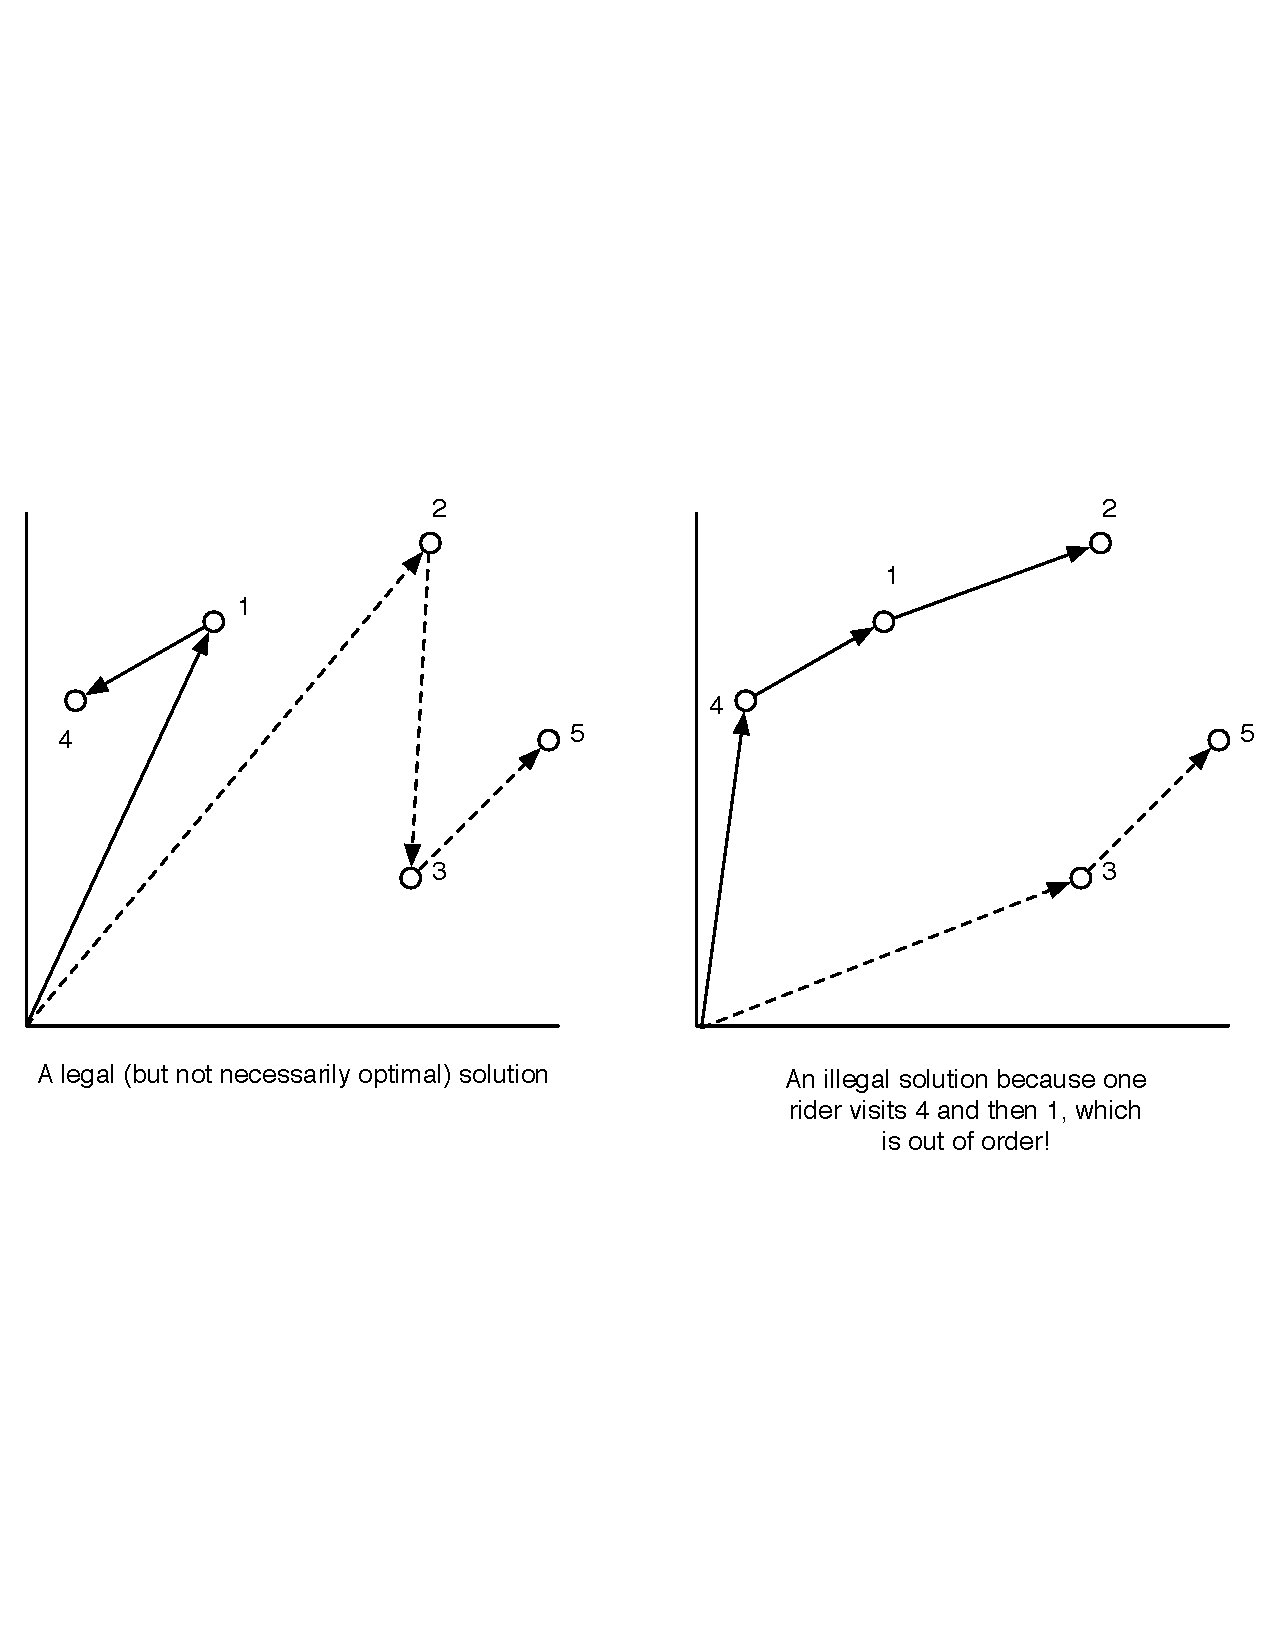
\includegraphics[height=2in]{WheelDeliver.pdf}
    \caption{Two examples of routes for the two riders.  The origin denotes the starting point $p_0$.  One rider's route is shown with solid lines and the other with dashed lines.  The route on the left is fair because points are visited by increasing indices.  The route on the right is not fair because, for example, point $p_4$  is visited before point $p_1$.}
  \end{figure}

  Jett and Anthony have hired you to design an efficient algorithm that takes as input an array of points $P = (p_1,p_2,\dots, p_n)$, sorted by the times in which their orders arrived, and outputs the sequences of delivery points for the two riders.

  Derive a recurrence relation, including base case(s), that is suitable for an efficient dynamic-programming solution for this problem.
  Briefly justify its correctness. You do not need to include pseudocode.

  \emph{Warning:} The most natural-seeming recurrences may have subtle errors!
      
  \begin{solution}
    
  \end{solution}
 
    
    
    



\end{questions}

\end{document}